%pdflatex -halt-on-error -aux-directory=tmp -output-directory=tmp rapport.tex%

\documentclass{article}
\usepackage{amsmath}
\usepackage[utf8]{inputenc}
\usepackage[T1]{fontenc}
\usepackage{graphicx}
\usepackage{hyperref}
\usepackage[francais]{babel}
\usepackage{listings}
\usepackage{xcolor}

\definecolor{codegreen}{rgb}{0,0.6,0}
\definecolor{codegray}{rgb}{0.5,0.5,0.5}
\definecolor{codepurple}{rgb}{0.58,0,0.82}
\definecolor{backcolour}{rgb}{0.95,0.95,0.92}

\lstdefinestyle{mystyle}{
    language=python,
    backgroundcolor=\color{backcolour},   
    commentstyle=\color{codegreen},
    keywordstyle=\color{magenta},
    numberstyle=\tiny\color{codegray},
    stringstyle=\color{codepurple},
    basicstyle=\ttfamily\footnotesize,
    breakatwhitespace=false,         
    breaklines=true,                 
    captionpos=b,                    
    keepspaces=true,                 
    numbers=left,                    
    numbersep=5pt,                  
    showspaces=false,                
    showstringspaces=false,
    showtabs=false,                  
    tabsize=2
}

\lstset{style=mystyle}

\title{Théorie des langages II}
\author{Wassim SAIDANE}
\date{01/03/2021}

\begin{document}
    \pagenumbering{gobble}
    \maketitle
    \pagenumbering{arabic}
    \section*{Note : }
    Ce cours est ma prise de note du cours de L3 infos de Théorie des langages II de Mamadou Kante
    \section*{Chapitre 1 : Langages algébriques (ou hors contexte)}
    \subsection*{\underline{1.1 Grammaires algébriques}}
    Une \textbf{grammaire algébrique} est un tuple $(V,\Sigma,R,S)$ où : \\
    \begin{itemize}
        \item $V$ : Ensemble fini, appelé ensemble de \textbf{varaiables} ou \textbf{non-terminaux}. 
        \item $\Sigma$ : Ensemble fini, appelé ensemble des \textbf{terminaux} $(\Sigma \bigcap V = \emptyset)$. 
        \item $S \in V$, appelé \textbf{non-terminal d'entrée (de départ)}. 
        \item $R$ est un ensemble de règles : \\
        \begin{equation*}
            R \subseteq P(V \times (V \bigcup \Sigma)^*)
        \end{equation*}
        chaque règle dans $R$ est écrite ainsi : 
        \begin{equation*}
            A -> w \text{         où       } A \in V, w \in (V \bigcup \Sigma)^*
        \end{equation*} 
    \end{itemize}
    Si $u,v,w \in (V \bigcup \Sigma)^* \text{  et  } A -> $\text(dérive)$ w \in R$. \\ 
    On dira que depuis $uAv$ on peut \underline{dériver} le mot $uwv$ et on note : $uAb \Longrightarrow uwv$ \\
    On dira $u$ dérive $v$, noté $u \Longrightarrow^* v$ \underline{si} 
    \begin{itemize}
        \item Soit $u=v$ 
        \item Soit il existe une séquance $u_1,u_2,...u_k$ tel que : \\
        \begin{equation*}
            u \Longrightarrow u_1, u_1 \Longrightarrow u_2, ... , u_i \Longrightarrow u_{i+1}, ... , u_{k-1} \Longrightarrow u_k, u_k \Longrightarrow v 
        \end{equation*}
    \end{itemize} 
    Le langage d'une grammaire G, notée $L(G)$, c'est l'ensemble $\{w \in \Sigma^* : S \Longrightarrow^* w\}$ \\
    \textbf{$L \subseteq \Sigma^*$ est algébrique si il existe une grammaire algébrique $G$ telle que $L=L(G)$}
    \newpage
    \underline{Exemples :} \\
    \begin{equation*}
        G=(\{S\},\{a,b\},R,S)
    \end{equation*}
    $uAv \Longrightarrow uwv$ si $A -> w$ \\
    \begin{equation*}
        \left.\begin{array}{rl}
            R: & S \rightarrow \varepsilon \\
            S & \rightarrow a S b \\
            S & \rightarrow S S
            \end{array}\right\} S \Rightarrow \varepsilon | SS  \mid  a S b
    \end{equation*}
    Des mots générés par cette grammaire : \\ 
    \begin{equation*}
        \varepsilon \text{(avec la règle S)} \rightarrow \varepsilon), ab (S \Longrightarrow aSb, aSb  \Longrightarrow ab)
    \end{equation*}
    \underline{Exemple 2 : }
    \begin{equation*}
        EA=(\{E,T,F\}, \{+,*,a,(,)\},R,\{E\}) 
    \end{equation*}
    \begin{equation*}
        E \rightarrow E+T \mid T 
    \end{equation*}
    \begin{equation*}
        T \rightarrow T*F \mid F
    \end{equation*}
    \begin{equation*}
        F \rightarrow (E) \mid a 
    \end{equation*}
    \underline{Mots générés : } $a+a*a, a+a+a*a, ... (a+a)*a$ \\
    \\
    A chaque fois qu'un mot est généré (ou dérivé) avec une grammaire, on peut lui associé un \underline{arbre de dérivation}, cet arbre décrit comment on construit le mot. \\
    La racine : C'est le non-terminal d'entrée. \\
    Les feuilles : Sont des terminaux. \\ 
    Les noeuds internes : Sont des non-terminaux. \\ 
    \\
    Si $A$ est un noeud interne, et on applique la règle $A \rightarrow w, w \in (V \bigcup \Sigma)^*$ \\ 
    Les fils de $A$ seront les lettres dans $V \bigup \Sigma$ qui composent le mot $w$. \\
    \underline{Exemple : } Avec la grammaire $EA$, on sait que $E$ gènère $a+a*a$. \\
    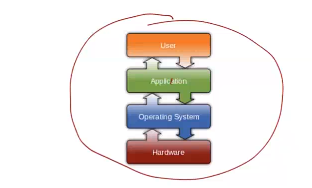
\includegraphics{capture/3.PNG} \\
    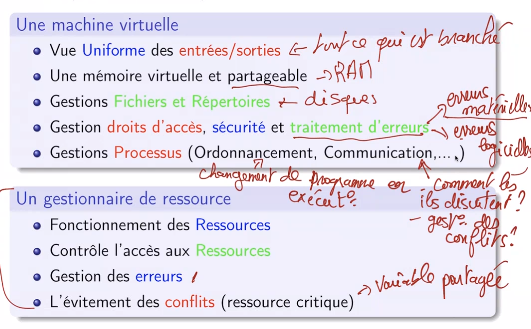
\includegraphics{capture/4.PNG} \\
    Un mot peut être dérivé de plusieurs façons différentes. Ceci peut induire un non-déterminisme sur la façon de savoir si un mot est généré par une grammaire. \\ 
    Une dérivation d'un mot (à partir d'une grammaire $G$) est une d\underline{dérivation gauche} si à chaque étape de la dérivation, on remplace la variable la plus à gauche. \\
    \\ 
    \underline{Définition 1.1 } Un mot $u$ est \underline{ambigüe} pour une grammaire $G$ si il existe deux dérivations gauches différentes du mot $u$ à partir de $G$. \\
    Une grammaire $G$ est dite anbigûe si elle admet un mot anbigüe. \\ 
    \\ 
    \underline{Proposition 1.1 : } On ne peut pas rendre non ambigüe toutes les grammaires. \\
    \underline{Preuve :} Montrer que toute grammaire reconnaissant le langage $\{a^ib^jc^k \mid i=j \text{ou} j=k\}$ est forcément ambigüe. \\
    \\
    Un langage tel que toute grammaire la générant est ambigüe est dite : Langage anbigüe.
    \newpage 
    Les différentes dérivations gauches d'un mot (à partir d'une grammaire) sont représentées par les arbres de dérivation. \\ 
    De façon équivalente, un mot est anbigüe si il admet deux arbres de dérivations différents. \\
    \subsection*{\underline{1.2 Forme Normale de Chomsky}} \\ 
    \underline{Définition 1.2 : } Une grammaire est en forme normale de Chomsky si chaque règle est de la forme : 
    \begin{equation*}
        A \rightarrow BC 
    \end{equation*}
    ou 
    \begin{equation*}
        A \rightarrow a
    \end{equation*}
    On accepte la règle $S \rightarrow \epsilon$ \\
    \\ 
    \underline{Théorème 1.1 : } Tout langage algébrique est le langage d'une grammaire en forme normale de Chomsky. \\
    
\end{document}
